\documentclass{article}
\usepackage{times}
\usepackage{cite}
\usepackage[margin = 1in]{geometry}
\usepackage{amsfonts, amsmath, amssymb}
\usepackage[none]{hyphenat}
\usepackage{fancyhdr}
\usepackage{listings}
\usepackage[nottoc,notlot,notlof]{tocbibind}
\usepackage{amsmath}  % for \text macro
\usepackage{amssymb}  % for \mathbb macro
\usepackage{graphicx}
\usepackage[spaces,hyphens]{url}
\usepackage[utf8]{inputenc}


\newtheorem{theorem}{Theorem}
\newenvironment{proof}{\noindent{\bf Proof:}}{$\hfill \Box$ \vspace{10pt}}  
\pagestyle{fancy}
\fancyhead{}
\fancyfoot{}
\fancyhead[L]{\slshape \MakeUppercase{Final year project}}
\fancyhead[R]{\slshape Feasibility Report}
\fancyhead[C]{\thepage}
\renewcommand{\footrulewidth}{0pt}
\parindent 0ex
\setlength{\parindent}{4em}
\setlength{\parskip}{1em}
\renewcommand{\baselinestretch}{1.5}
\begin{document}
\begin{titlepage}
\begin{center}
\vspace*{1cm}
\begin{figure}[h!]
\centering

\includegraphics[scale=0.5]{logo}
\end{figure}
\Large\textbf{System Requirement Specifications}\\
\Large\textbf{Final Year Project}\\
\vfill
\line(1,0){400}\\[1mm]
\huge{\textbf{SmartGuide: A smart campus guide using BLE based indoor localization}}\\[3mm]
\line(1,0){400}\\
\vfill

\large{Rida Mahmood  (2016-CE-54)}\\
\large{Tooba Naseer  (2016-CE-72)}\\
\large{Rabeya Hamood  (2016-CE-81)}\\
\large{Ayesha Jabbar  (2016-CS-159)}\\

\large{Supervised by: Dr. Sheikh Faisal Rasheed}\\
\large{Co-advisor : Dr. Beenish Ayesha Akram}\\
\large{\textbf{Department of Computer Science and Engineering}}\\
\large{\textbf{University of Engineering and Technology, Lahore}}\\
\end{center}
\end{titlepage}
\tableofcontents
\thispagestyle{empty}
\clearpage
\setcounter{page}{1}

\makeatletter
\newcommand{\heading}[1]% #1 = text
{\par\vskip 1.5ex \@plus .2ex
 \hangindent=1em
 \noindent\makebox[1em][l]{$\,\bullet$}\textbf{\large #1}%
\par\vskip 1.5ex \@plus .2ex
\@afterheading}
\makeatother

\section{Overview of Project}
Outdoor and indoor localization is an integral component of  IoT (Internet of Things) in this era of mobile computing. Indoor localization can open new horizons for ubiquitous applications targeting university departments, government small institutes, software houses, airports, shopping malls, museums etc. Our project will find the location of a specific person by using appropriate machine learning approach using BLE based Android application. This location will be used to provide guided tour of the indoor building (Computer Science and Engineering Department at UET, Lahore) we will use to validate our work. 
\\\\
This project will guide persons who are not much familiar with visiting place. It has an android application that will predict the indoor location of a person at room level and also gives information of current room location and nearby rooms in the form of text, images, audio and videos. In our case visiting place will be CSE dept at UET LHR. For room prediction, RSSI fingerprints of BLE beacons will be captured for training of model. After finding the location of the person, guidelines of that certain room/area will be provided to the user on user end Android application. Indoor positioning has numerous applications. We can use indoor positioning of people to guide them inside shopping malls, airports or museums. 


\subsection{Background}
Outdoor localization has been formalized by using satellite-based technologies i.e. GPS\cite{GPS}, BeiDou\cite{cooper2016loco}, GLONASS\cite{cooper2016loco}, and GALILEO\cite{GALILEO}. It is hard for finding the indoor location by using conventional GPS technology because of no direct (Line of Sight)\cite{akram2018censloc} in indoors, so we cannot use these technologies for indoor positioning. Up to date, the technologies used for indoor localization approach are: TOA (Time of Arrival), TDOA (Time Difference of Arrival), AOA (angle of arrival) but they have some limitations. TOA and TDOA require precise clock count and its synchronization and AOA-based systems require special antennas for their propagation. So, we are going to implement a system which employs suitable machine learning approach to find the location by using RSSI (Received Signal Strength Indicator) fingerprinting technique. This RSSI values will pass to the trained model (a model which is trained on a given set of input and output values by using appropriate machine learning algorithm) which gives the location of the mobile device.
\subsection{Motivation}
People/visitors who go to an unknown place find it difficult to traverse and wants to find places/people of interest easily. Such problems motivate us to provide ease and leverage facility to users so that they can see the information of a particular indoor environment on his mobile application automatically. BLE is available on nearly every smart device so no additional hardware required at user end. Hence by utilizing their indoor location determined using machine learning on BLE fingerprints, guided tours of smart campus to visitors can be provided and facilitating them. We are using latest technology of BLE beacons because they work on battery and consume less energy than Wi-Fi signals\cite{hultgren2015evaluating}.

\subsection{Scope}
In this project, android application runs on a user’s mobile device and and will capture BLE RSSI fingerprints. The fingerprints collected at the initial stage will be processed and used to train suitable machine learning model, after training of the ML based location prediction model, based on the room prediction relevant information of nearby rooms, facilities and personnel available will be prepared to be displayed to user at run time , the user will be guided to install our Android app on their phone, their mobile device will capture BLE fingerprint and the fingerprint will be sent to back end server where our trained model will predict their current location inside building in terms of room\cite{Loco}. The relevant information will be delivered and shown on user mobile device providing guided tour. 
The placement of Bluetooth low energy beacons will be held in CSE dept at UET Lahore. 

\subsection{Problem Statement}
Whenever a visitor goes to university campus or visits a new place, he does not know about the specifications of that area i.e. what happens in that specific room or what courses have been taught in a particular and its nearby labs. So, we are developing a system which assists them in determining the textual and pictorial information of a particular area and its nearby locations. For this purpose, we first find the indoor location of a user by using BLE beacons and RSSI values, and then provide information to him automatically on his Android application. 
\subsection{Possible Applications of work}
The possible application of work for our project are as follows:


\begin{itemize}
\item Software house information (Development, QA, Frontier)
\item Airport assisting system
\item University Campus smart information system
\item Government small Institutes
\item Medical departments exploration in hospitals
\end{itemize}

\section{Overall Description}
\subsection{Product Context}
\begin{itemize}
\item It navigates the user location
\item It also give the user’s nearby location
\item It provides information of the current location of user i.e. the room’s pictures and in textual description it will tell about the office hours or if it is a lab then how many teachers are teaching in that lab and the schedule.
\item User can see that if his nearby place is room or lab. It will provide the room number and pictures.
\item Most of us don’t use guide boards because it is time consuming. This app will navigate you to your required lab.

\end{itemize}
\subsection{User Characteristic}
\begin{center}
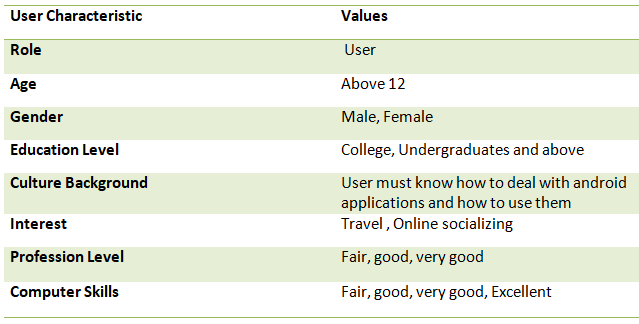
\includegraphics[scale=0.8]{userch}
\\Figure 13: User Characteristics
\end{center}

\subsection{Constraints}
\begin{itemize}
\item It only tells the indoor location of CSE department because we need BLE beacons for deployment which predict room location. Actually, BLE beacons are very expensive. That’s why, it is implemented in specific area. 
\item User can only use this app for CSE department.
\item This app cannot tell about the outdoor location.
\item Only visitors and new student of CSE department use this app.s
\item If we have more resources such as BLE beacons, we can enhance the scope of the project such as we can implement this in other departments and other locations. 
\item We are not providing information in video form.

\end{itemize}


\subsection{Assumptions and Dependencies}
\begin{itemize}
\item We can implement our project in different departments of UET.
\item Even we can also implement this application in shopping malls, Offices and other universities.
\item We can also provide information in video format in this app.
\item We can introduce the concept of indoor localization for whole world.
\end{itemize}

\section{Existing System}
\subsection{Comparison of Existing Systems}
The smart campus guided tour based on indoor localization is not implemented yet, also there are little or even no research specifically focus on the smart campus guided tour based on indoor localization. There exist a research that presents a mobile campus tour application based on augmented reality in various universities and the features of application are the information about points of interest, location search and navigation, but it provides outdoor locations of large university campus using GPS, because it is not based on room level prediction and information about indoor locations. But there are a lot of researches that provide different methodologies for room level prediction. In recent years, indoor localization systems have great significant research activity and growing interest for their great expected social impact. In spite of the numerous research advances, no proper solutions have yet defined. The diversity and heterogeneity of applications, scenarios, sensor and user requirements make it difficult to create uniform solutions. There are multiple solutions present in research area for room level prediction\cite{wei2018end}. Here are the comparisons of few of them:


\begin{center}
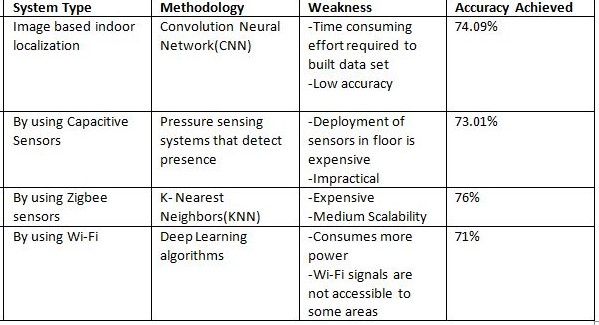
\includegraphics[scale=0.8]{abc}
\\Figure 1: Comparison of Existing Systems
\label{fig:five}
\end{center}

\subsection{Drawbacks of Existing Systems}
There are many drawbacks in existing systems. In some systems, camera is required for indoor positioning which is obtrusive for some users. High cost and effort is required for the deployment of indoor localization infrastructure. Most of the existing systems have medium or low accuracy. In image based indoor localization, time consuming effort is required for built data sets. Wi-Fi fingerprinting is relatively better than other systems because of finding position by using already deployed infrastructure. But its main drawback is that it consumes more power. There are some spots where Wi-Fi access points would be difficult to power. There are some areas where Wi-Fi signals are not accessible. In our proposed system, we will find indoor location using BLE beacons. BLE beacons are small in size, light weight and cheaper then Wi-Fi. BLE consumes less power than Wi-Fi. BLE beacons are usually battery powered, which are more flexible and easier deployed than sensors used by existing systems. BLE RSS signals can have a higher sample rate than Wi-Fi RSS signals (0.25 Hz~2 Hz). Our proposed system will provide more accuracy than existing systems and also it is unobtrusive. So, our proposed system will overcome the shortcomings in existing systems. Furthermore, our system will not only predict location but also provide information of that location and nearby location in form of text, videos, audio and images which is missing in existing systems because they find indoor positioning for different purposes\cite{zhuang2016smartphone}.
\section{Software Development Life Cycle Used}
To implement a project, one must have to follow some software development life cycle to deliver his project completely according to user requirements in time. By following a certain SDLC, a project developer feels so comfortable as he have specific tasks and time to implement project timely  which meets the user’s point of view. In our project, there are lots of fluctuations time by time. So, we decided to follow AGILE model.
\subsection{AGILE SDLC}
Agile SDLC model is a combination of incremental and iterative process models deals with customer requirements satisfaction and process adaptability by rapid delivery of working product to the customer. This model breaks the whole project in small modules. Do proper testing after completion of each module. Then deliver this working module to the customer and important stakeholders to satisfy them. If that module doesn’t meet their point of views properly or to which customer point of view as he didn’t explained in the document, then it has to be iterated to fulfill their new recommendations. And the other perspective is that if the customer wants to add some functionality in that particular module then a developer has to follow an incremental technique to add specific functionalities. 
To complete each deliverable module of the project, developer has to follow these steps
\begin{itemize}
\item Planning
\item Requirements Analysis
\item Design
\item Coding
\item Unit Testing and
\item Acceptance Testing
\end{itemize}

\begin{center}
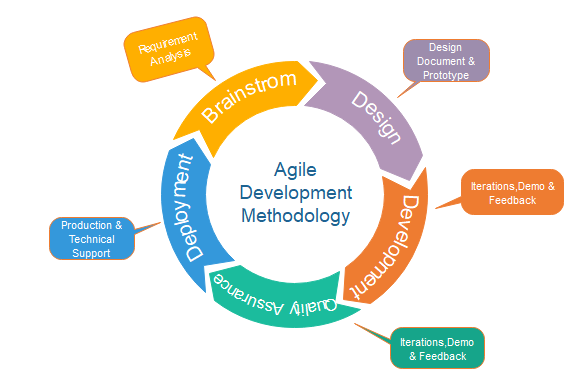
\includegraphics[scale=0.6]{agile}
\\Figure 2: Agile Methodology
\end{center}
\subsection{Justification for AGILE SDLC}

These steps will justify that our project is based on agile methodology:
\begin{itemize}
\item All the requirement specifications and the scope of the project is strictly defined in our documentation but by the time, it may require some amendments, so they will change by ourselves.
\item Planning of time, design, implementation and testing is done.
\item Hardware and software parts of our project are specified into a work breakdown structure.
\item All the Modules of our project are divided in small pieces of time according to estimated time.
\item In model training module, we first use Weka and then following TensorFlow to meet the requirements; hence we followed an incremental and iterative model.
\item Do unit and acceptance testing after completion of each module.
\item Budget plan for our project is defined
\item We Add functionality of delay in Data Capturing application  which capture data after some seconds when a user change his indoor location.
\item Add restart functionality to restart scanning of Bluetooth devices once it stops which leads to incremental change in data capturing application.
\item Roles and responsibilities of team members vary according to the prescribed task and time limit.
\end{itemize}

\section{Requirement Analysis}
The most important section of system requirement specification document is requirement analysis. To start any project, anyone needs to know his system requirements. This section includes all the software, hardware functional requirements of our system, user interfaces, database diagram, use case diagram, use case tests and test cases. Basically, we will discuss all the specifications of our system.
\subsection{Hardware Functional Requirements}
\heading{Deployment of BLE beacons}
Deployment of BLE beacons on the ceiling is the requirement to capture fingerprints of BLE beacons with different mobile devices. At what angle and at what part of the ceiling these beacons should display, all we get it know before their deployment.
\subsection{Software Functional Requirements}
\subsubsection{Data Capturing Application}
\heading{Bluetooth scanning for nearby devices}
A scanning function is made in data capturing application to scan BLE beacon for nearby mobile devices. Devices who present/locate near a certain BLE beacon are being scanned.

\heading{Capture RSSI values for nearby beacons}
BLE beacons Bluetooth range exists in a certain region and this region contain different mobile devices far and near to BLE beacon depending upon their indoor location. So, this function will capture RSSI fingerprints for all mobile devices which being scanned in that certain region.
\heading{Add delay factor to capture FP’s}
Once fingerprints of certain mobile device have been captured at a particular location and by determining the indoor location, we provide room information through our application to a user’s mobile device. The user may change his indoor location after a while. To provide updated room information to the user we are making a delay function which captures user fingerprints after a certain time (seconds) and provide him updated information according to his room location.
\heading{Automatic restart Bluetooth scanning for nearby devices once it stops}
Automatic restart scanning function will scan for BLE beacon nearby mobile devices once scanning has been stops, because in this way our system will able to automatically find coming and going devices in a particular region and provide rooms information accordingly.
\heading{Generate .csv file for each BLE beacon}
After capturing the fingerprints of all devices with a single BLE beacon which lie in that certain region, this function will generate .csv file and RSSI values of all devices in that file.
\textbf{\textbf{
\subsubsection{SmartGuide: Android Application}}}
The functional requirements of our system for User are as follows:
\heading{Load trained model in Android app}
There is need to load machine learning trained model in our Android application to predict the room location of a particular person.
\heading{Get the prediction of room from trained model}
When a trained model receives .csv file of a particular BLE beacon, it gives the particular roomID of that beacon to a mobile device which is receiving higher RSSI value from that BLE beacon.

\heading{Allow user to know his indoor location}
This function will enable users to see their indoor location i.e. in which room they are.
\heading{Fetch information of that particular room}
This function will send RoomID of a particular BLE beacon to the database from which room information in image, texts and audio format can be fetched.

\heading{Provide information of the room to the user}
After fetching the information of a particular room, this function becomes enable and displayed that information on user mobile screen.
\heading{Enable user to get information of nearby rooms}
This function allow users to see their nearby (left, right, front and back) rooms and textual and pictorial information about that rooms.
\\\\ The functional requirements of our system for Admin are as follows:

\heading{Allow admin to SignUp for our application}
To use an Android application, in this case admin has to register on our application to add, update and delete records of certain data in our application.
\heading{Provide account activation functionality to the admin}
Admin can login on another device; he has no restriction to use our application on a certain device. He may be login or logged out.
\\
\heading{Admin has all the records of data}
Admin has the ability to get all up-to-date records of data. Data can be of staff members, their visiting hours, room information, lab accessories and much more.
\heading{Store information to database in images, audios and text format of rooms and their nearby rooms}
This function will store information about rooms in images, audios and text format in the database. Also, the information about nearby rooms of a certain room will also be stored by the admin in the database manually.

\heading{Allow admin to edit or update the information about rooms}
When After sometime, the specifications and in formations about certain rooms and departments can be changed. So, this function will enable admin to update the information accordingly to provide up-to-date information to the user.
\heading{Admin has all those functionalities which a user has}
Admin can see the information of a room and nearby rooms in any format provided in our application like user.

\subsection{Non Functional Requirements}
\heading{Reliability}
Our project will be reliable .The user’s information will be kept confidential and there will be no worry of losing the information.
\heading{Usability}
Our application will be usable for the users and easy to use.
\heading{Maintainability}
This system will have the capability to adapt changes and amendments done in the database by the admin as the information of rooms will be updated or edited.
\heading{Security}
Our Android application will work under potential risks. It will not be accessible by the malicious user or be crashed by external attacks.
\heading{Recoverability}
In case of crash, our system information will recoverable
\heading{Safety}
Optimize safety in the design, development, use and maintainability of the application.
\heading{Reusability}
Our system will provide reusability factor to the visitors of the department.
\heading{Performance}
To make a system which gives accurate and up-to-date information about rooms even a user change his indoor location after a while. This system will give results efficiently in small time.


\subsection{Hardware Interfaces}
BLE beacons are bluetooth low energy beacons. Classic bluetooth consumes more power than BLE beacons and 
transmits to long ranges. On the other hand, BLE consuming much less power because it transmits data over the small range.Bluetooth having version greater than 4.0 are BLE.BLE Beacon is a tiny device with a massively used for broadcasting of signals. It has unique ID. A beacon has three major components: a small ARM computer, a Bluetooth Smart connectivity module and batteries for powering the entire circuit. 
The CPU of the ARM computer has an antenna attached to it. It broadcasts electromagnetic waves with specific lengthand frequency. We develop Data Capturing Application that will interface with beacons in order to capture the signal strength of BLE beacons in the form of RSSI values.
These RSSI values further used for the prediction of room.
\\

\heading{Bluetooth Low Energy Beacons}
\begin{center}
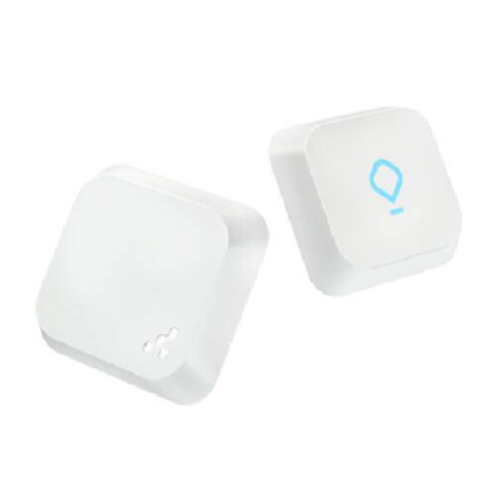
\includegraphics[scale=0.35]{beacon1}
\\Figure 3: BLE beacons
\end{center}
\pagebreak

\heading{Interfacing with Beacons}
\begin{center}

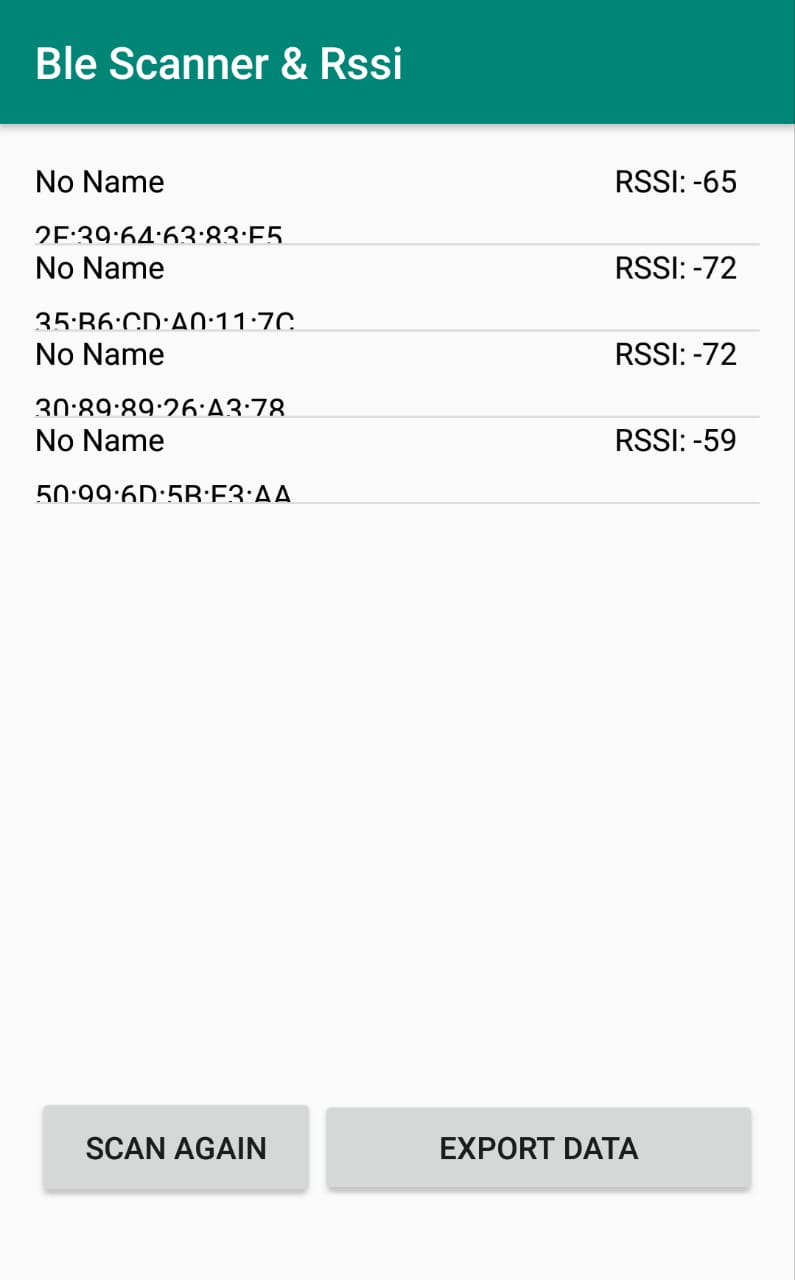
\includegraphics[scale=0.25]{hi}
\\Figure 4: Data Capturing Application
\end{center}

\subsection{Communication Interfaces}

\begin{center}

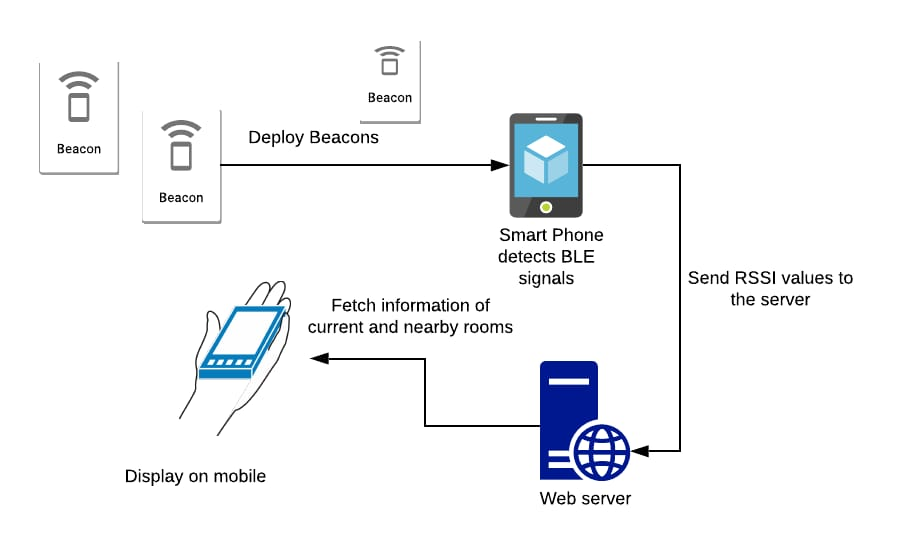
\includegraphics[scale=0.3]{ci}
\\Figure 5: Communication Interface
\end{center}

\subsection{User Interfaces}

\heading{Splashig Screen}
\begin{center}

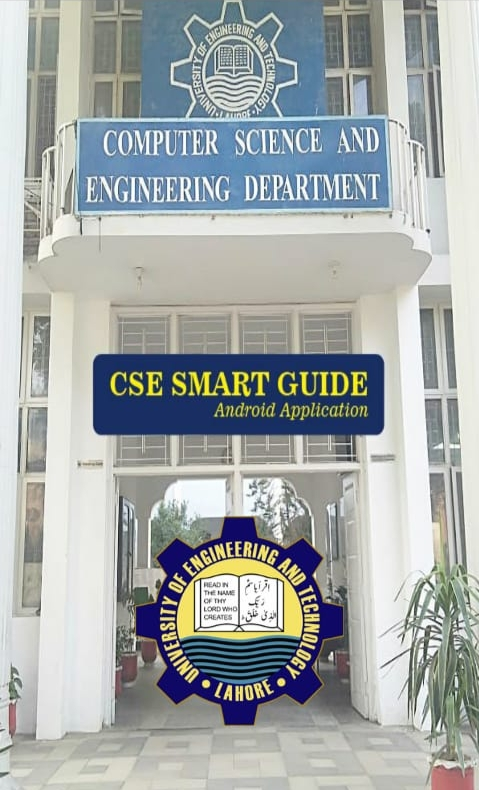
\includegraphics[scale=0.3]{f1}
\\Figure 6: Splashing Screen
\end{center}
\heading{Screen 1}
\begin{center}

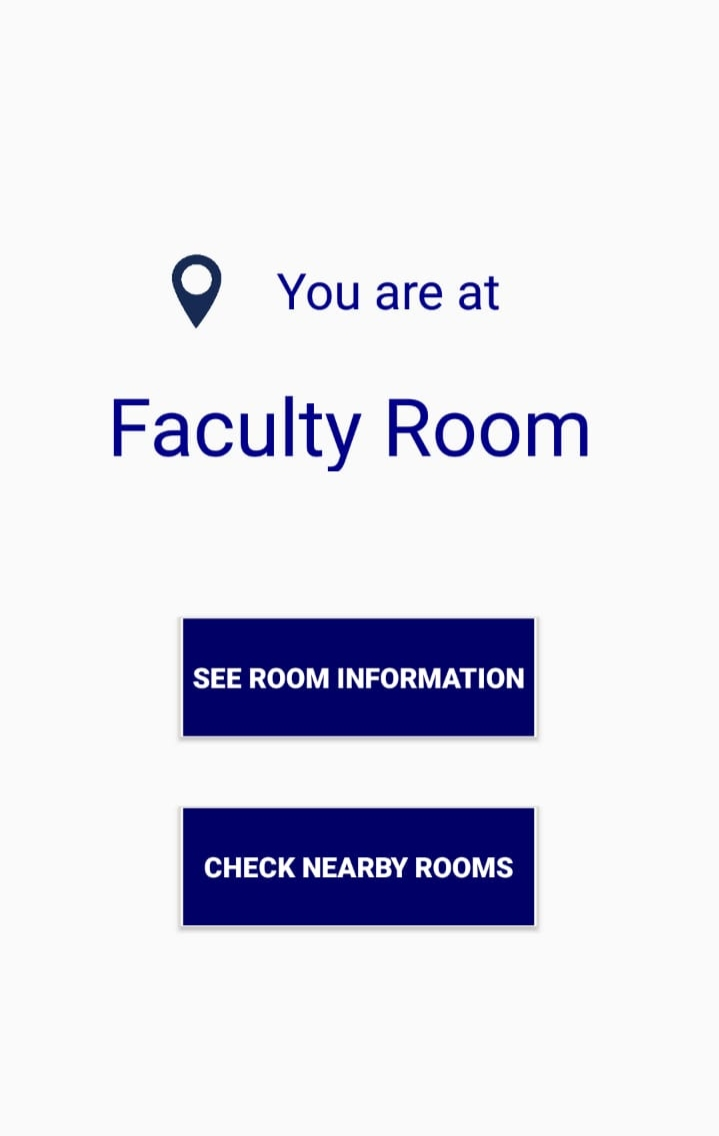
\includegraphics[scale=0.2]{f2}
\\Figure 7:Prediction of Room
\end{center}
\heading{Screen 2}
\begin{center}
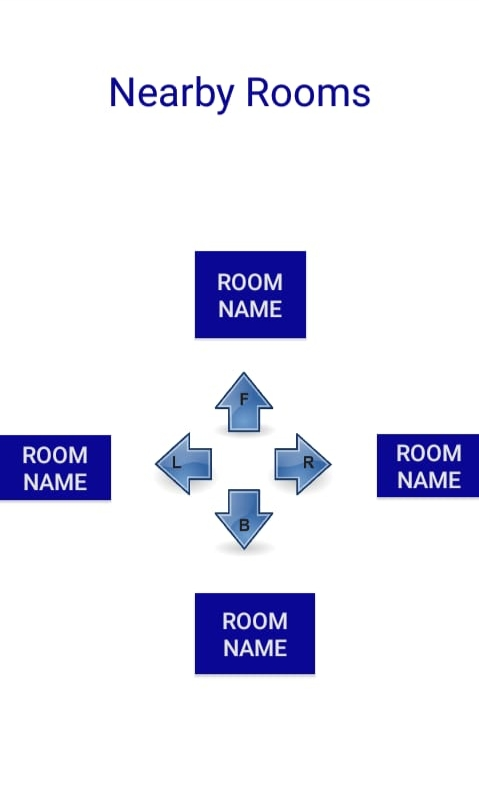
\includegraphics[scale=0.3]{f3}
\\Figure 8: Nearby Rooms
\end{center}
\heading{Screen 3}
\begin{center}
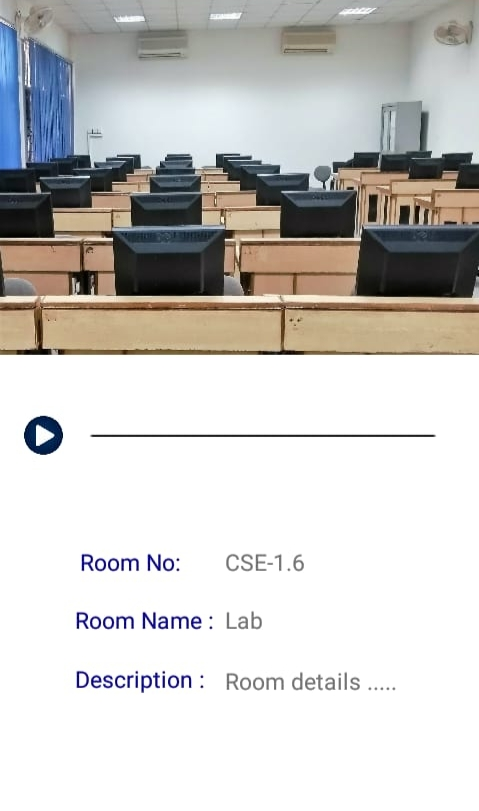
\includegraphics[scale=0.35]{f4}
\\Figure 9: Room Information
\end{center}
\heading{Screen 4}
\begin{center}
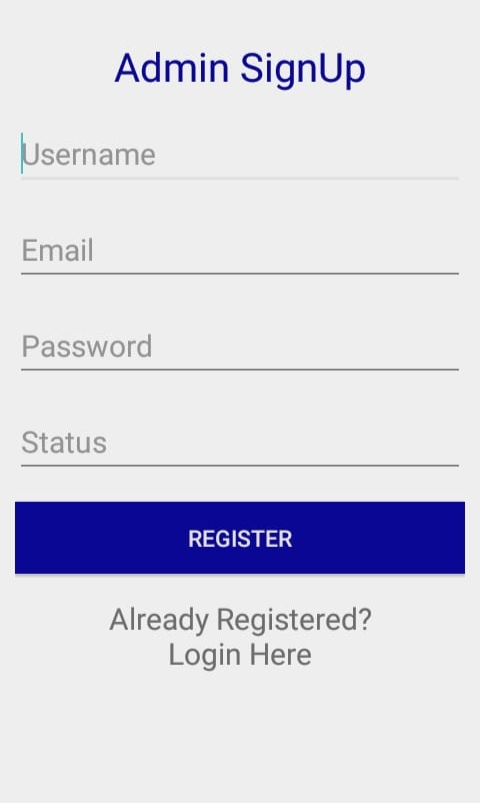
\includegraphics[scale=0.32]{f5}
\\Figure 10: Admin SignUp
\end{center}
\heading{Screen 5}
\begin{center}
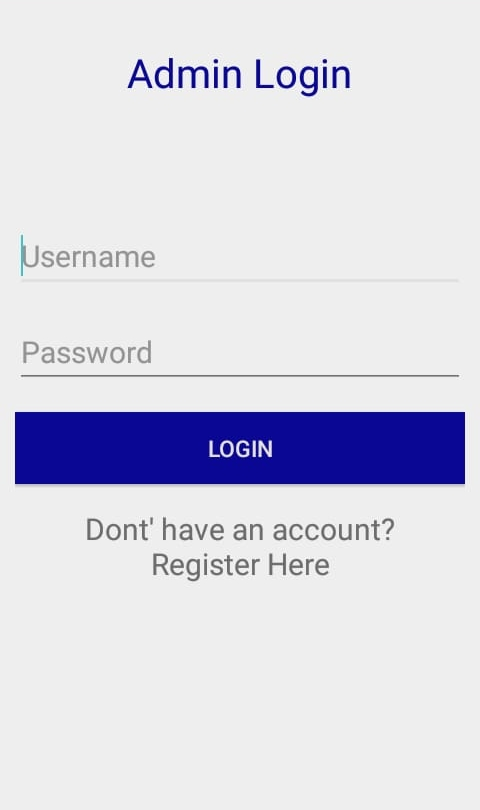
\includegraphics[scale=0.32]{f6}
\\Figure 11: Admin LogIn
\end{center}
\heading{Screen 6}
\begin{center}
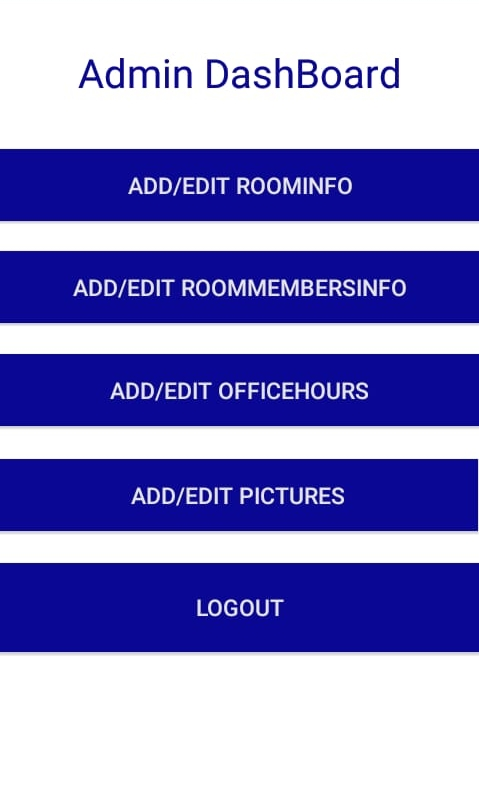
\includegraphics[scale=0.3]{f7}
\\Figure 12: Admin Tasks
\end{center}
\heading{Screen 7}
\begin{center}
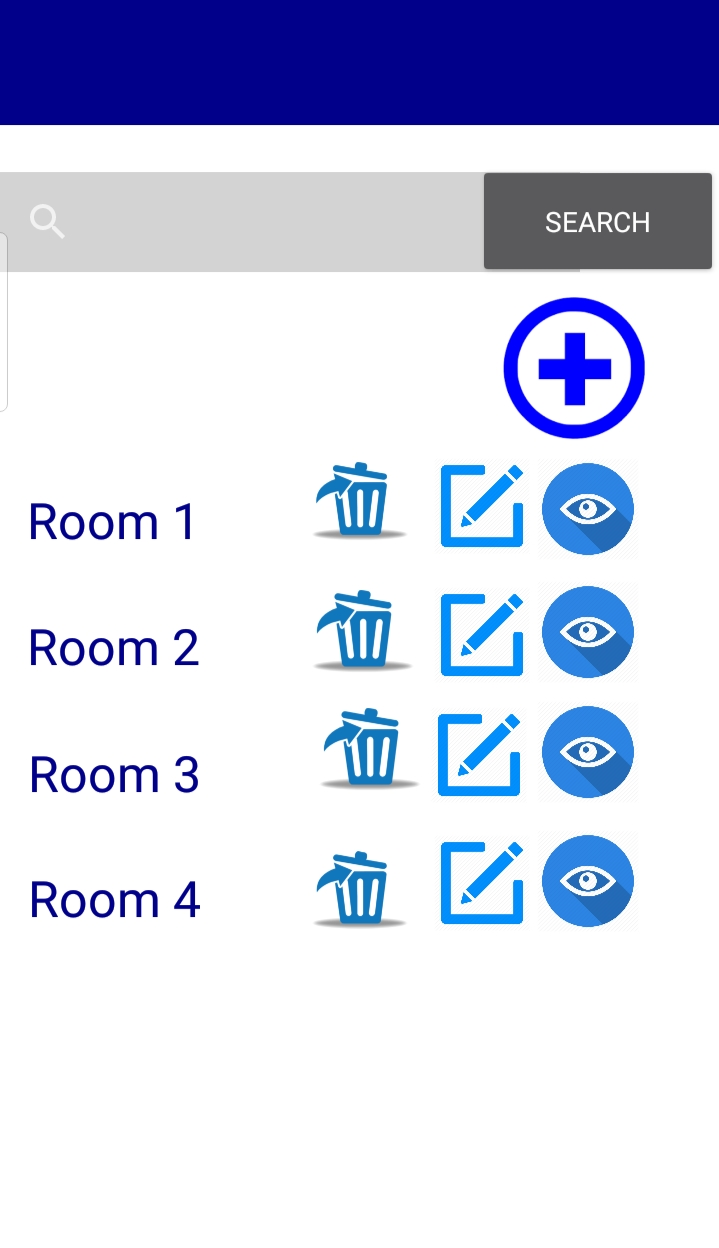
\includegraphics[scale=0.20]{f8}
\\Figure 13: Room Index
\end{center}
\heading{Screen 8}
\begin{center}
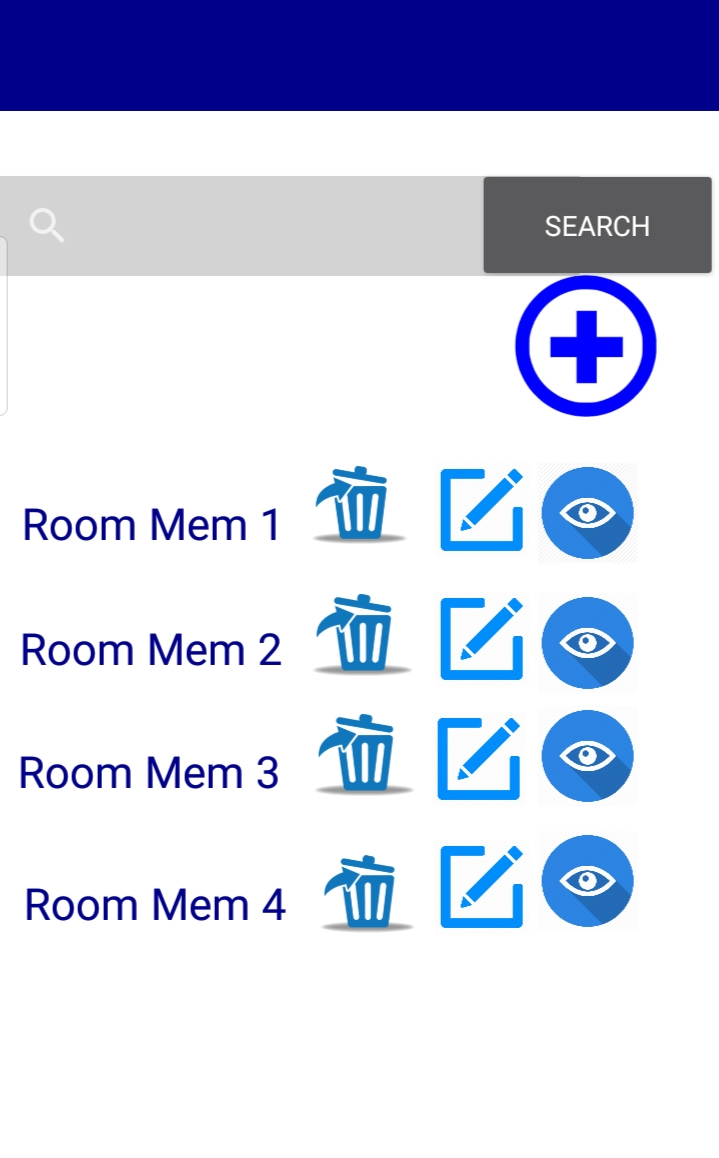
\includegraphics[scale=0.20]{f9}
\\Figure 14:Room Members Index
\end{center}
\heading{Screen 9}
\begin{center}
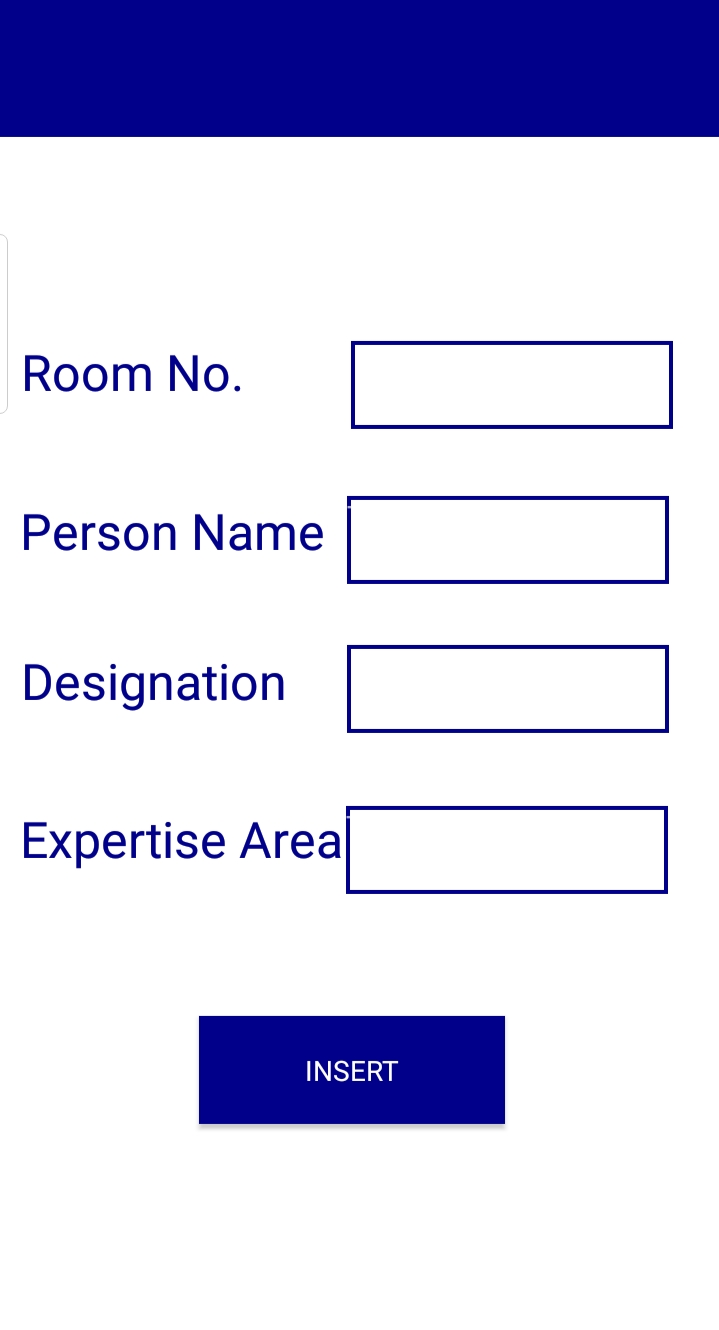
\includegraphics[scale=0.20]{f10}
\\Figure 15: Addition and editing of room members information
\end{center}
\heading{Screen 10}
\begin{center}
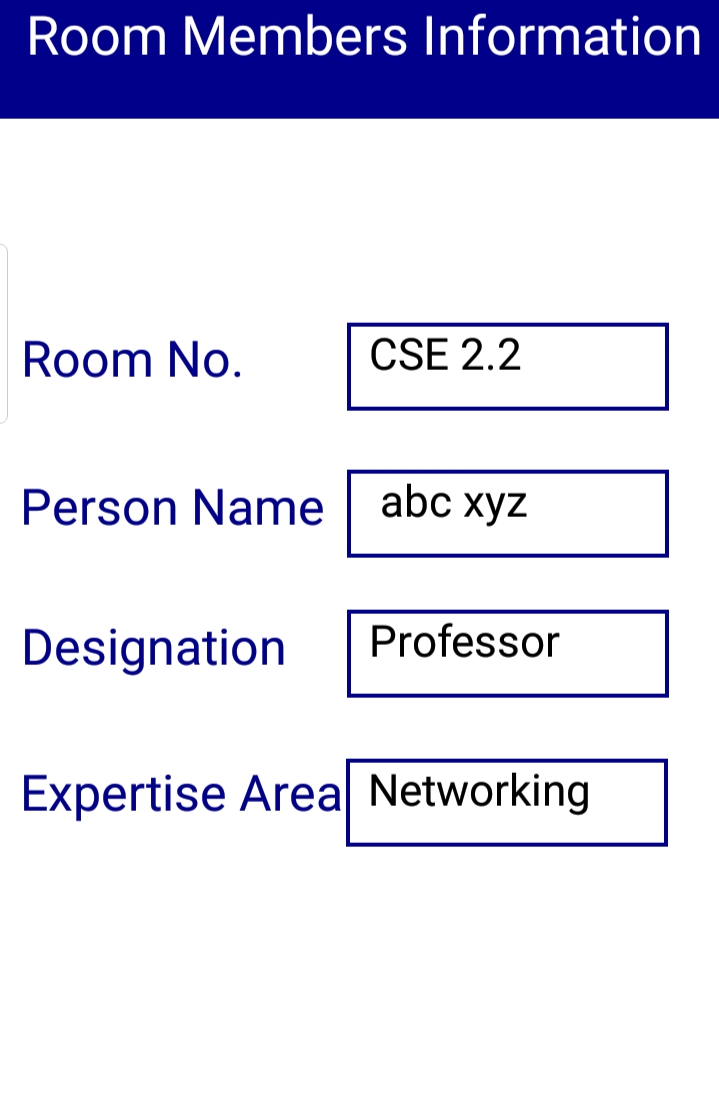
\includegraphics[scale=0.20]{f11}
\\Figure 16: View room members information
\end{center}
All other interfaces for Admin of modifying office hours, pictures information are similar to above interfaces.

\subsection{Use Case Diagram}
\begin{center}
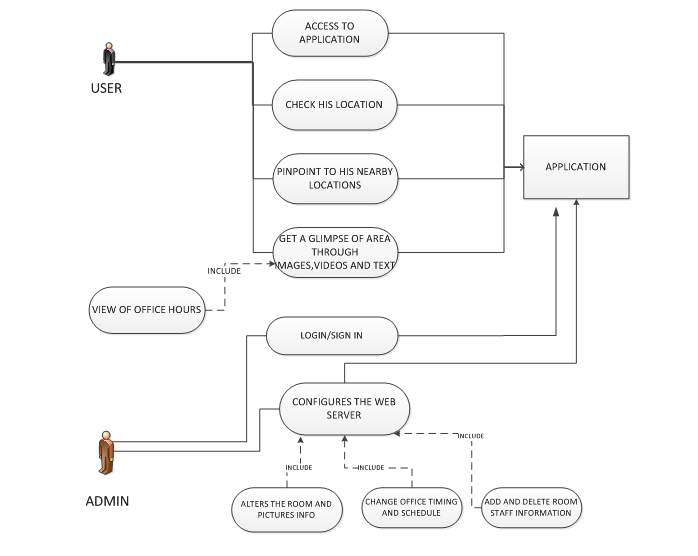
\includegraphics[scale=0.8]{usecase}
\\Figure 17: Use Case Diagram
\end{center}
\subsection{Use Case Texts}
\begin{center}
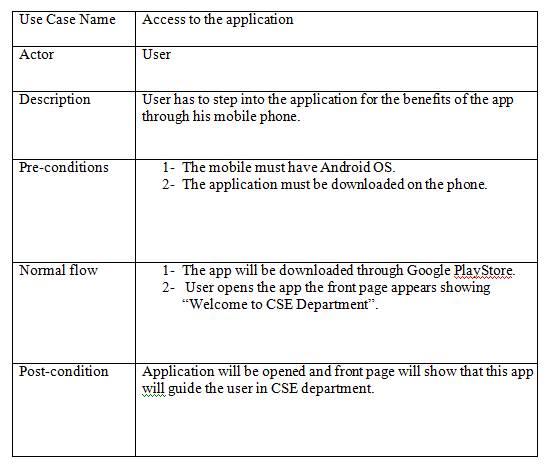
\includegraphics[scale=0.8]{uc1}
\\Figure 18: Use Case 1
\end{center}
\begin{center}
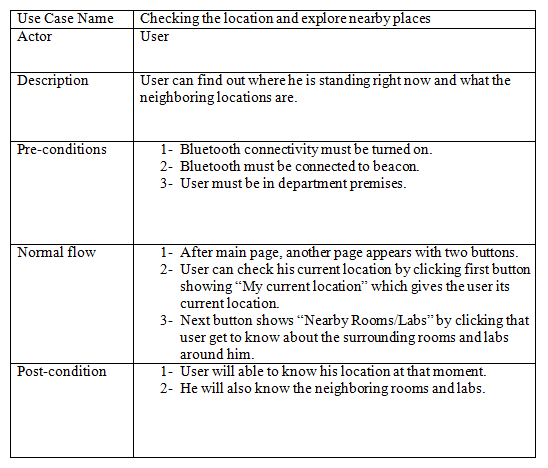
\includegraphics[scale=0.8]{uc2}
\\Figure 19: Use Case 2
\end{center}
\begin{center}
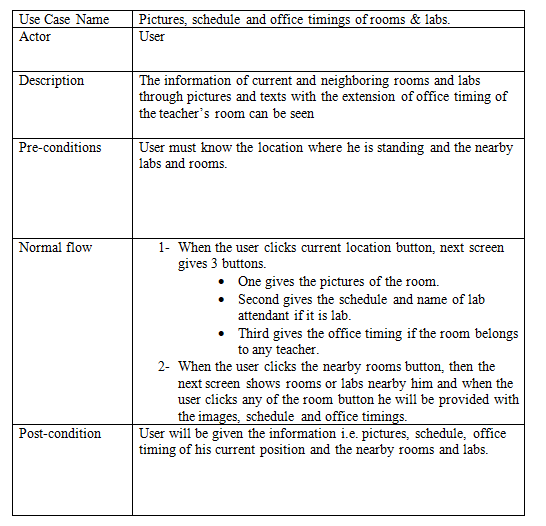
\includegraphics[scale=0.8]{uc3}
\\Figure 20: Use Case 3
\end{center}
\begin{center}
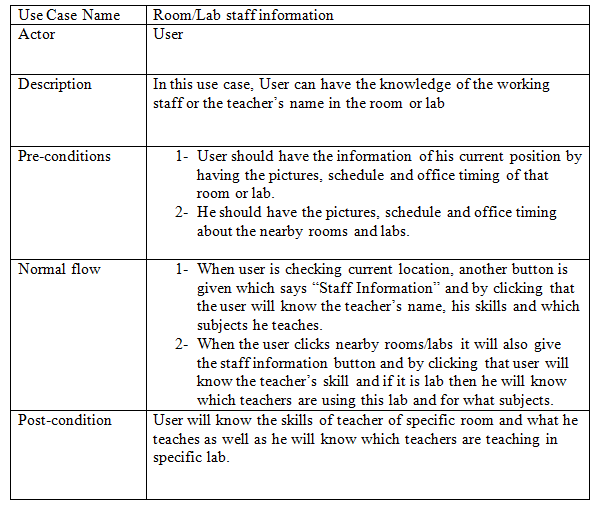
\includegraphics[scale=0.7]{uc4}
\\Figure 21: Use Case 4
\end{center}
\begin{center}
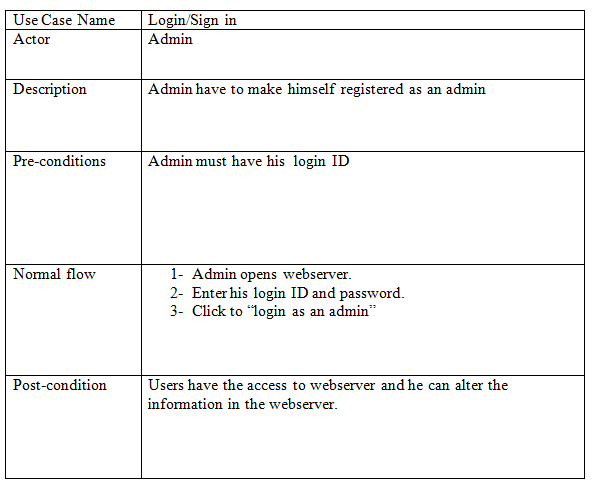
\includegraphics[scale=0.77]{uc5}
\\Figure 22: Use Case 5
\end{center}
\begin{center}
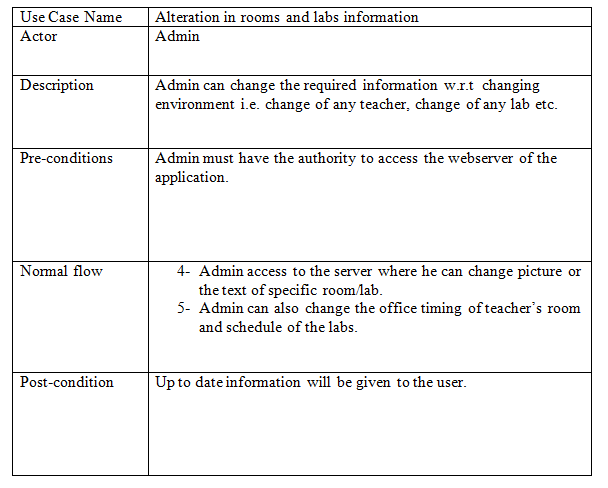
\includegraphics[scale=0.75]{uc6}
\\Figure 23: Use Case 6
\end{center}
\begin{center}
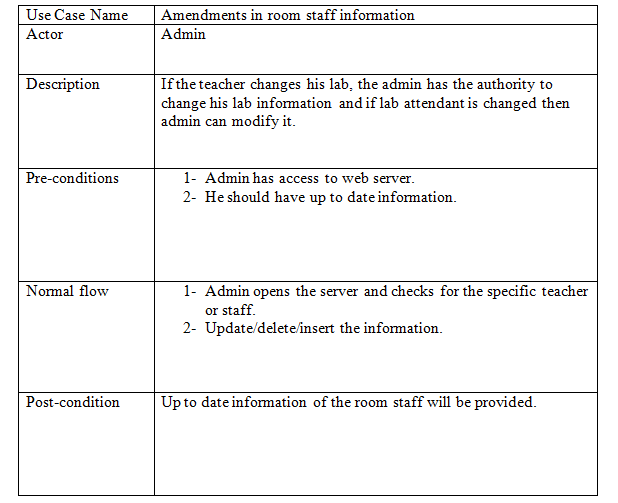
\includegraphics[scale=0.75]{uc7}
\\Figure 24: Use Case 7
\end{center}
\subsection{Test Cases}
\begin{center}
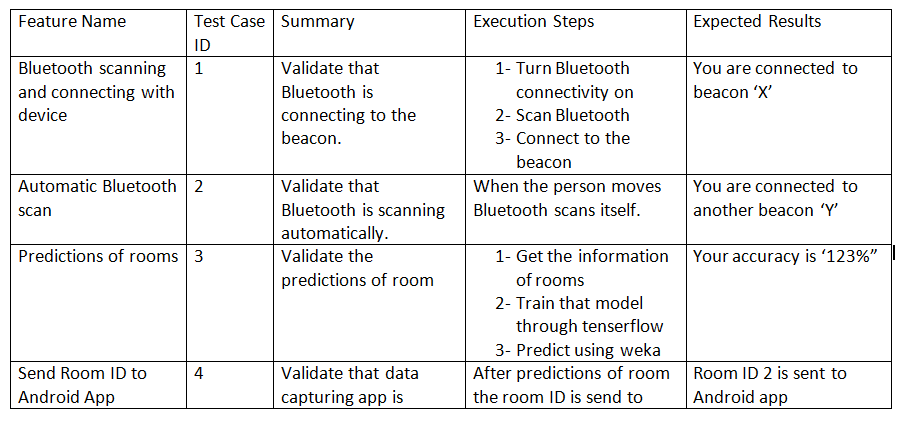
\includegraphics[scale=0.8]{tc1}

\end{center}
\begin{center}
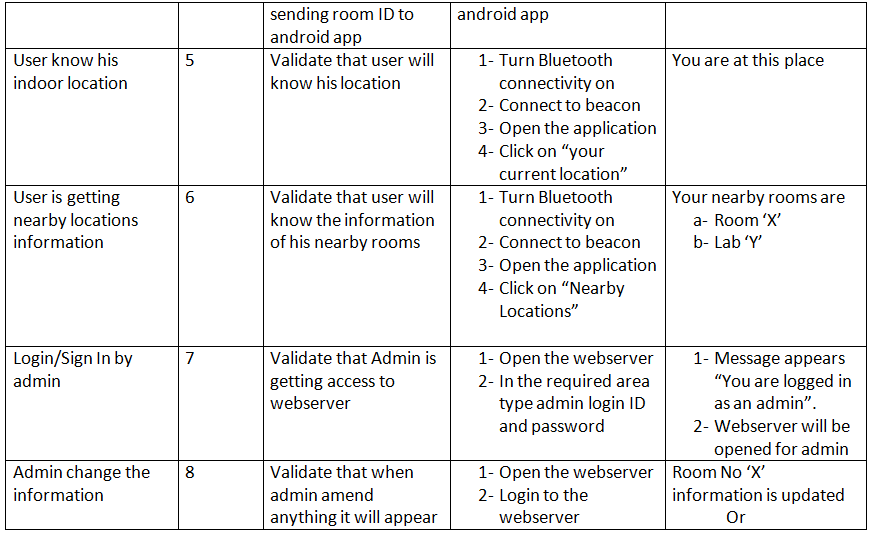
\includegraphics[scale=0.8]{tc2}

\end{center}
\begin{center}
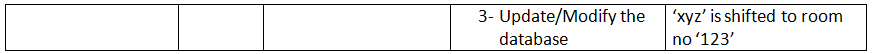
\includegraphics[scale=0.8]{tc3}
\end{center}

\section{Planning}
\subsection{Milestones}
\begin{center}
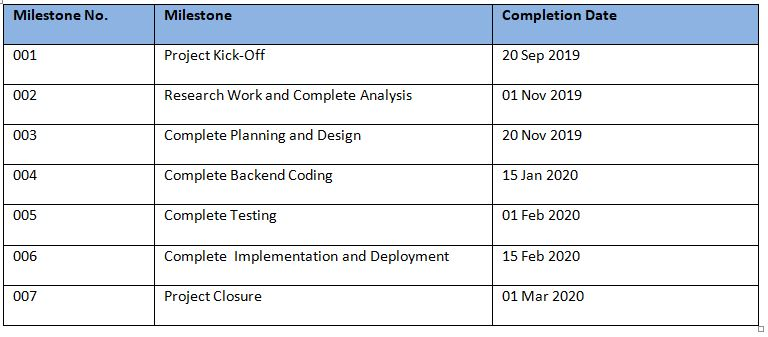
\includegraphics[scale=0.8]{milestone}
\\Figure 25: Milestones
\end{center}
\subsection{Work Breakdown Structure}
\begin{center}
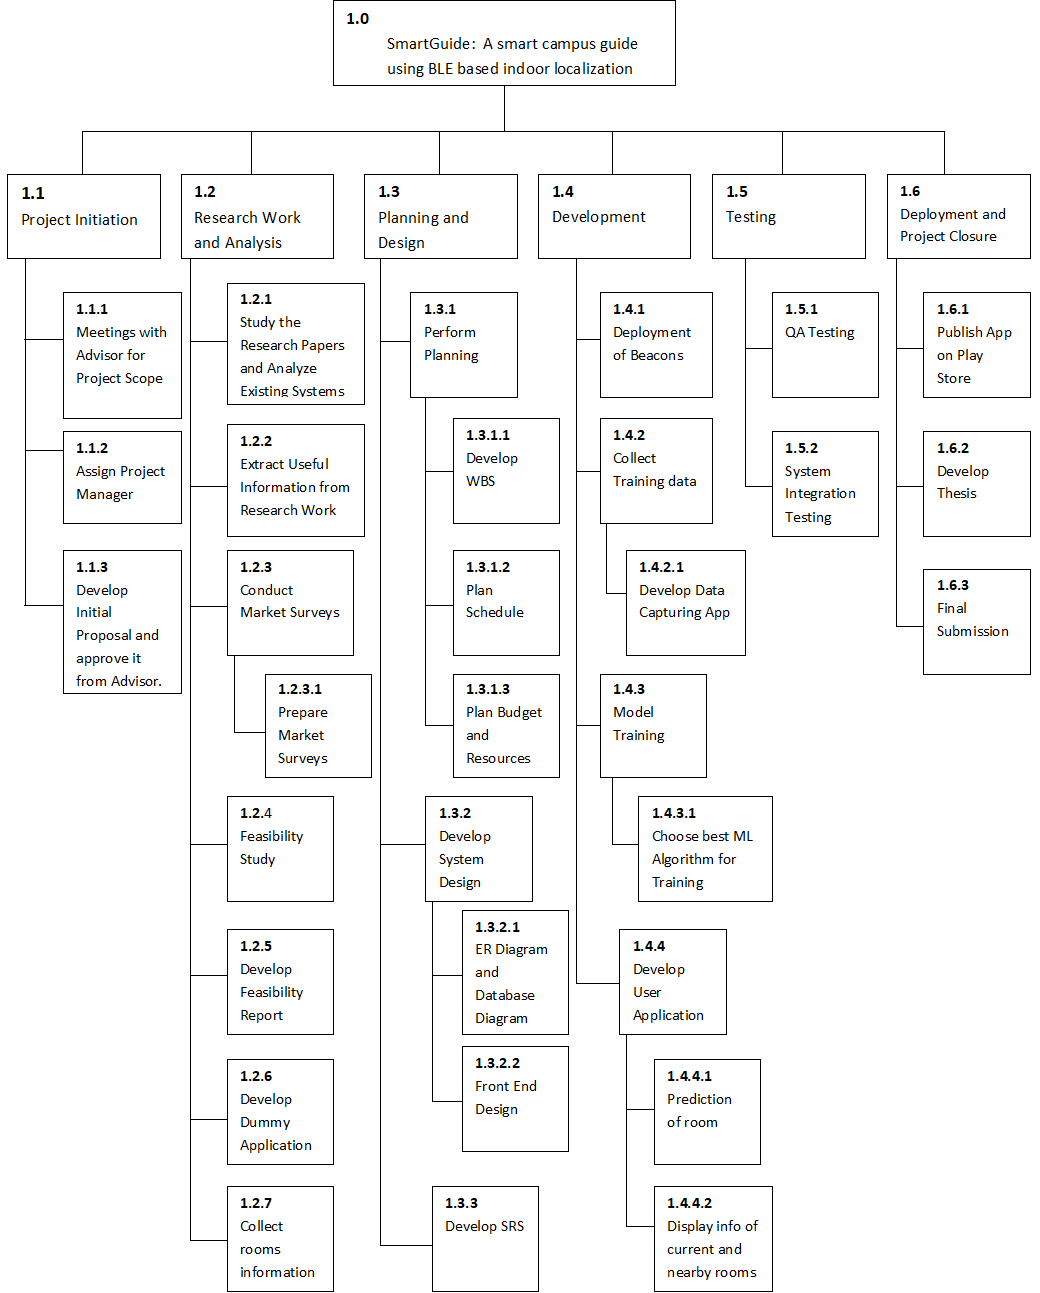
\includegraphics[scale=0.6]{WBS}
\\Figure 26: Work Breakdown Structure
\end{center}
\subsection{Network Dependency Diagram}
\begin{center}
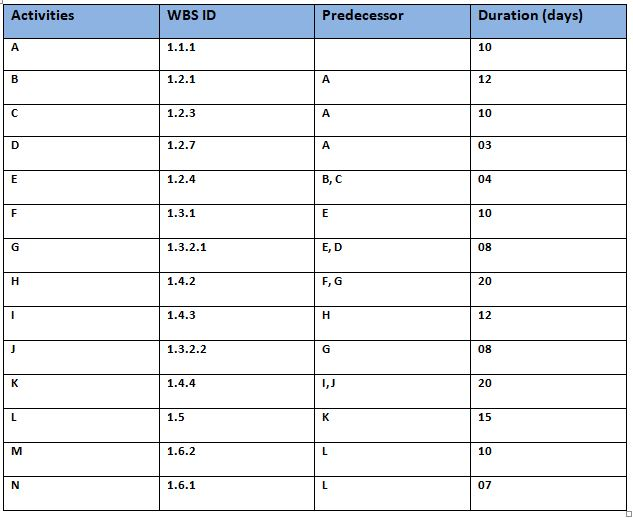
\includegraphics[scale=0.8]{nddtable}
\\Figure 27: Network Dependency Diagram Table
\end{center}
\begin{center}
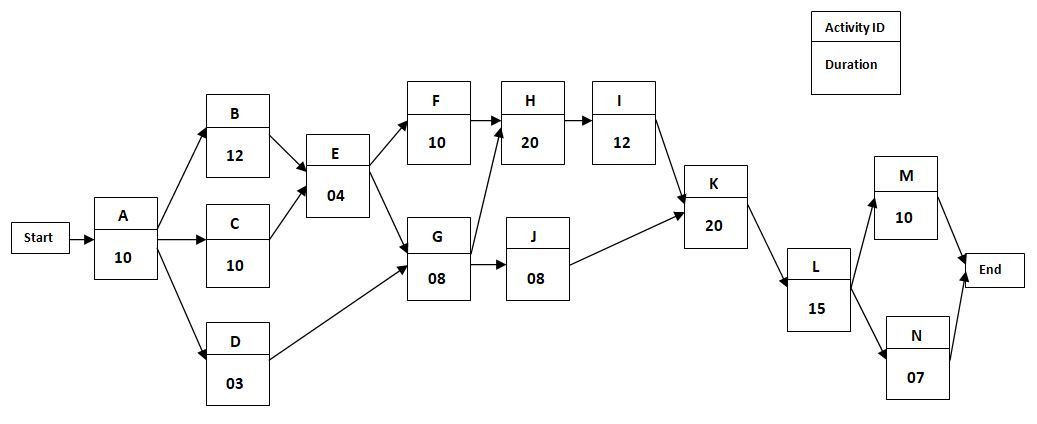
\includegraphics[scale=0.6]{ndd}
\\Figure 28: Network Dependency Diagram
\end{center}
\subsection{Gantt Chart}
\begin{center}
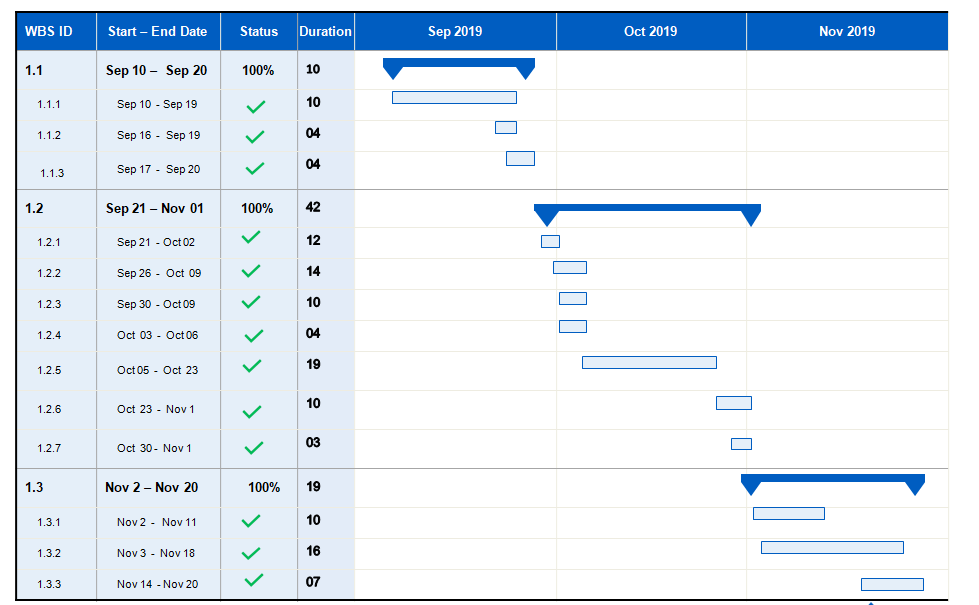
\includegraphics[scale=0.6]{gc1}
\\Figure 29: Gantt Chart
\end{center}
\begin{center}
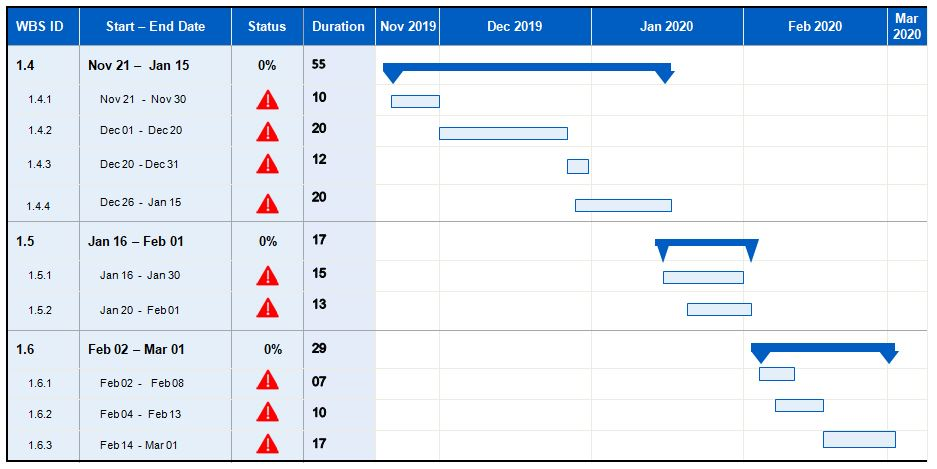
\includegraphics[scale=0.6]{gc2}
\\Figure 30: Gannt Chart
\end{center}
\section{Design}
\subsection{Data Flow Diagram}
\begin{center}
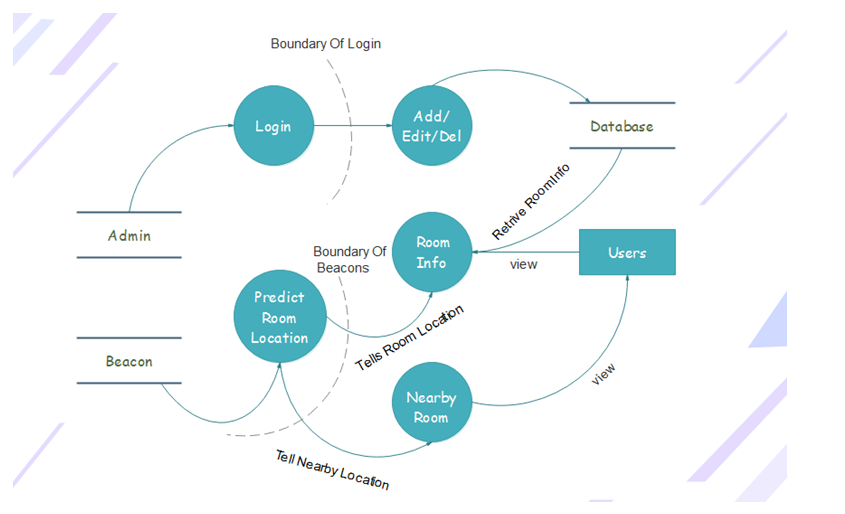
\includegraphics[scale=0.8]{dfd}
\\Figure 31: Data Flow Diagram
\end{center}
\subsection{Activity Diagram}
\begin{center}
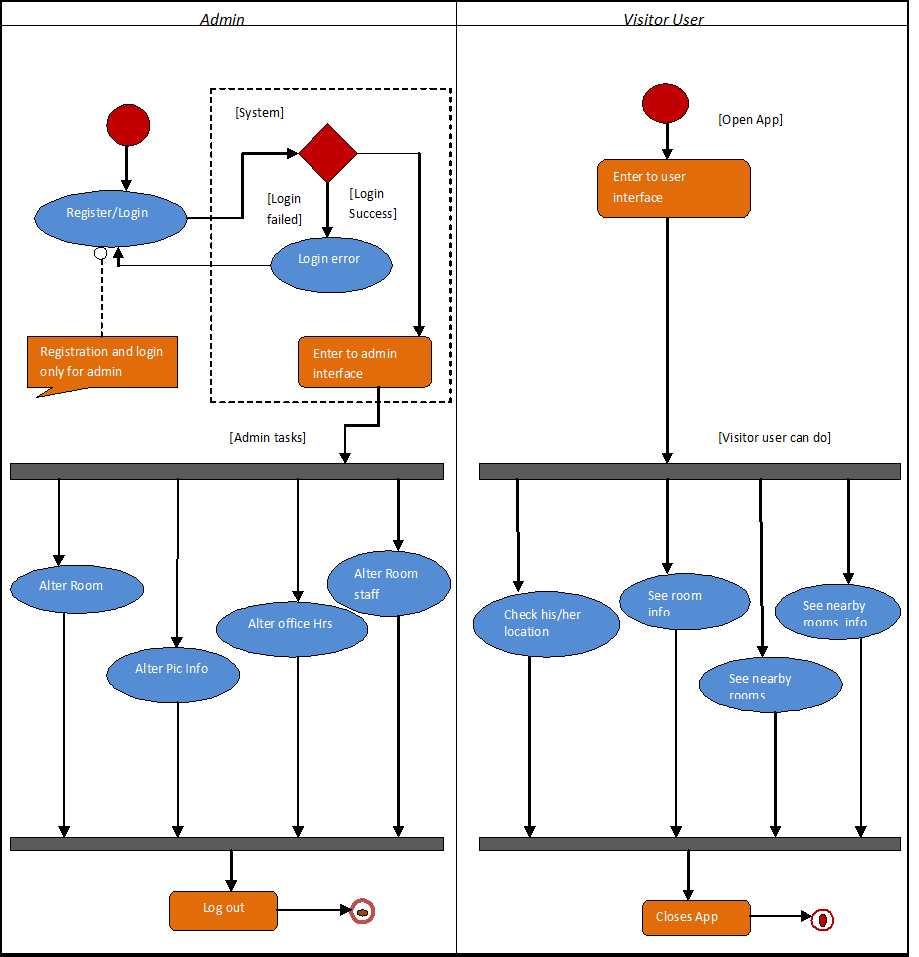
\includegraphics[scale=0.6]{ad}
\\Figure 32: Activity Diagram
\end{center}
\subsection{Data Modeling}
\subsubsection{ER Diagram}
\begin{center}
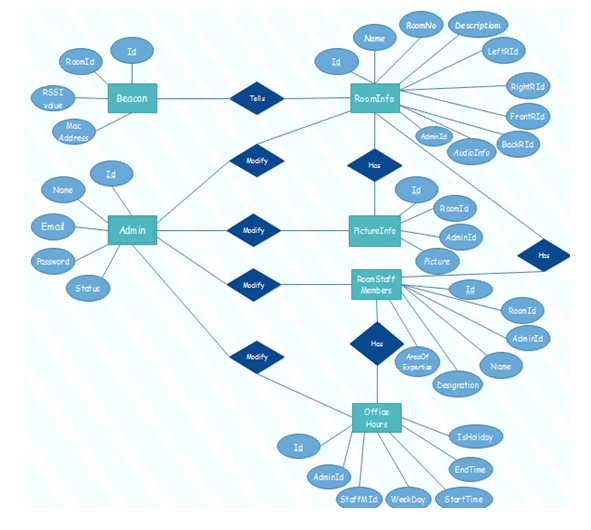
\includegraphics[scale=1.0]{erd}
\\Figure 33: ER Diagram
\end{center}

\subsubsection{Database Diagram}
\begin{center}
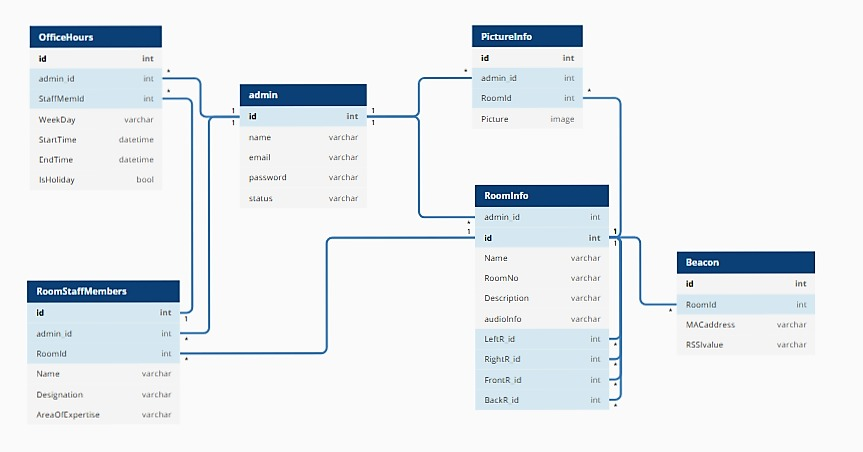
\includegraphics[scale=0.6]{dbd}
\\Figure 34: Database Diagram
\end{center}
\subsection{Class Diagram}
\begin{center}
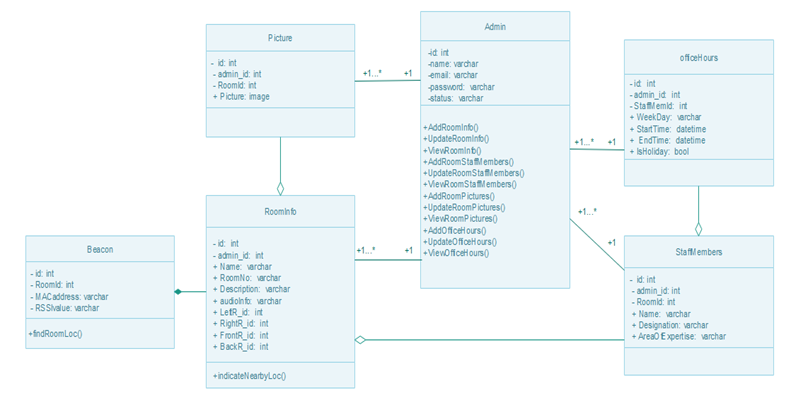
\includegraphics[scale=0.7]{cd}
\\Figure  35:Class Diagram
\end{center}
\pagebreak
\section{References}


\bibliographystyle{plain}
\bibliography{References}
\end{document}